\documentclass{article}

% if you need to pass options to natbib, use, e.g.:
% \PassOptionsToPackage{numbers, compress}{natbib}
% before loading nips_2018

% ready for submission
\usepackage[final]{nips_2018}

% to compile a preprint version, e.g., for submission to arXiv, add
% add the [preprint] option:
% \usepackage[preprint]{nips_2018}

% to compile a camera-ready version, add the [final] option, e.g.:
% \usepackage[final]{nips_2018}

% to avoid loading the natbib package, add option nonatbib:
% \usepackage[nonatbib]{nips_2018}

\usepackage[utf8]{inputenc} % allow utf-8 input
\usepackage[T1]{fontenc}    % use 8-bit T1 fonts
\usepackage{hyperref}       % hyperlinks
\usepackage{url}            % simple URL typesetting
\usepackage{booktabs}       % professional-quality tables
\usepackage{amsfonts}       % blackboard math symbols
\usepackage{amsmath}       % blackboard math symbols
\usepackage{amssymb}       % blackboard math symbols
\usepackage{nicefrac}       % compact symbols for 1/2, etc.
\usepackage{microtype}      % microtypography
\usepackage{color}
\usepackage{natbib}
\usepackage{algpseudocode,algorithm,algorithmicx}

\usepackage{graphicx}
\graphicspath{{figures/}}

\usepackage{tikz}
\usepackage{pgffor}
\usetikzlibrary{arrows,positioning}

% My commands
\newcommand{\R}{\mathbb{R}}
\newcommand{\E}{\mathbb{E}}
\newcommand{\TODO}[1]{\textcolor{red}{\textbf{TODO: #1}}}

\newcommand{\cA}{\mathcal{A}}
\newcommand{\cH}{\mathcal{H}}
\newcommand{\cL}{\mathcal{L}}
\newcommand{\cN}{\mathcal{N}}
\newcommand{\cO}{\mathcal{O}}
\newcommand{\cS}{\mathcal{S}}
\DeclareMathOperator*{\argmax}{argmax}


\title{Learning an abstract system identification space for adaptive online control}

% The \author macro works with any number of authors. There are two
% commands used to separate the names and addresses of multiple
% authors: \And and \AND.
%
% Using \And between authors leaves it to LaTeX to determine where to
% break the lines. Using \AND forces a line break at that point. So,
% if LaTeX puts 3 of 4 authors names on the first line, and the last
% on the second line, try using \AND instead of \And before the third
% author name.

\author{
  James A.~Preiss, Karol Hausman, Gaurav S. Sukhatme\thanks{Use footnote for providing further
    information about author (webpage, alternative
    address)---\emph{not} for acknowledging funding agencies.} \\
  Department of Computer Science\\
  University of Southern California\\
  Los Angeles, CA 90089\\
  \texttt{japreiss@usc.edu} \\
  %% examples of more authors
  %% \And
  %% Coauthor \\
  %% Affiliation \\
  %% Address \\
  %% \texttt{email} \\
  %% \AND
  %% Coauthor \\
  %% Affiliation \\
  %% Address \\
  %% \texttt{email} \\
  %% \And
  %% Coauthor \\
  %% Affiliation \\
  %% Address \\
  %% \texttt{email} \\
  %% \And
  %% Coauthor \\
  %% Affiliation \\
  %% Address \\
  %% \texttt{email} \\
}

\begin{document}
% \nipsfinalcopy is no longer used

\maketitle

\begin{abstract}
  The abstract paragraph should be indented \nicefrac{1}{2}~inch
  (3~picas) on both the left- and right-hand margins. Use 10~point
  type, with a vertical spacing (leading) of 11~points.  The word
  \textbf{Abstract} must be centered, bold, and in point size 12. Two
  line spaces precede the abstract. The abstract must be limited to
  one paragraph.
\end{abstract}

\section{Introduction}

Reinforcement learning (RL) is a highly general framework for learning policies that make decisions sequentially in an environment.
RL is an attractive approach to robotic control problems
because the same learning algorithm and model structure can be applied to a wide range of robot environments without requiring per-environment manual effort or insight.
Yet, in contrast to the generality of RL itself,
the policies trained with RL are usually highly specialized and fail to generalize to other similar environments, even when the differences are small. \TODO{citation. Who said ``we're testing with the training set''?}

Overfitting to the training environment is problematic if we desire to deploy a trained policy on other systems without re-training.
Training in a fast simulator and deploying on a real robot can save lots of time,
an important consideration due to high sample complexity of most RL algorithms.
However, simulators that run faster than real-time cannot faithfully reproduce complex physical phenomena such as fluid dynamics or collision and friction forces.
If a robot manufacturer wishes to train a policy in a lab and deploy it on mass-produced robots,
they must account for manufacturing variations that will affect dynamics.

%A significant body of work attempting to bridge the reality gap has emerged in recent years.
Failure to generalize has been the subject of intense attention from the RL community.
Randomization of textures and colors in the visual input has been used for successful sim-to-real transfer
for indoor quadrotor navigation~\citep{sadeghi-cad2rl-rss17}
and grasping objects on a table~\citep{tobin-domainrand-arxiv17}.
However, these methods use high-level control inputs and hand-engineered low-level controllers to abstract away some of the physical detail.
In contrast, we target systems where the learned policy has direct control over the actuators, and can thus access the full abilities of the system.

In this paper, we design an architecture and training regime that is capable of producing diverse behaviors that vary widely depending on the dynamics parameters,
rather than ``lowest common denominator'' behaviors that are adequate for a range of dynamics but optimal for none.

Many other works (\TODO{cite}) focus on adapting between a simulation with fixed dynamics parameters and a single real robot.
In contrast, in this paper we attempt to train in simulation a policy that can transfer to many different real-world systems.

We are motivated by the following observation:
The end goal is for the policy to behave near-optimally in reality.
Identifying the true system dynamics parameters is unnecessary work.
Instead, our scheme learns an abstract space that is both
1) useful to help the policy to behave optimally in simulation, and
2) easy to identify from a short state-action trajectory.

\section{Related Work}
Work addressing the reality gap can largely be separated into two categories:
those that attempt to improve the \emph{a priori} generalization performance of the policy without any data from the test environment,
and those that establish some link between the training and test environments \emph{a posteriori} after collecting some data from the test environment.

The most straightforward \emph{a priori} approach is domain randomization,
in which the parameters of the dynamics and/or observations are randomized during training.
Randomization of textures and colors in the visual input has been used for successful sim-to-real transfer
for indoor quadrotor navigation~\citep{sadeghi-cad2rl-rss17}
and grasping objects on a table~\citep{tobin-domainrand-arxiv17}.
Dynamics randomization has shown good results in~\citet{antonova-pivoting-corr17} \TODO{other good citations for this}.
\TODO{ensemble approaches (no resampling).}
However, these methods implicitly assume that, given the observable states,
there exists an action distribution that will produce acceptable behavior over all possible values of the hidden, randomized states.

%Ensemble approaches \TODO{}
%\citet{mordatch-ensemble-icra15} employed a fixed ensemble of models with perturbed parameters for trajectory optimization and controller synthesis for complex humanoid robots.
%\TODO{is this level of detail necessary?}

In cases where this assumption is violated, the policy must be able to behave differently in different environments,
and there must be a mechanism to extract some information about the hidden parameters of the environment during interaction.
This is the scenario considered in this paper.
A similar approach to ours is~\citet{yu-up-osi-rss17},
where the authors trained a policy that takes the dynamics parameters as input
and an online system identification module to estimate them.
We observe that estimating the true dynamics parameters is more work than needed--
we can instead learn to map the dynamics parameters into an embedding space
that is more useful for the policy, as well as being easier to estimate.
~\citet{peng-dynamics-randomization-corr17} make a similar observation and use a recurrent policy architecture.
A recurrent architecture is able to extract information about the environment in its internal state without imposing any particular structure on the information that is extracted.
By comparison, our framework makes it possible to modify the training reward such that the model is explicitly encouraged to behave in a manner that makes the parameters easily observable.

Model-agnostic meta-learning (MAML)~\citep{finn-maml-icml17} is another \emph{a priori} approach.
MAML learns a policy that can adapt to the test environment in a single gradient descent step after gathering a small amount of data.
\TODO{what is our comparison to MAML.}



The \emph{a posteriori} approach has been widely deployed in visual domains
using generative adversarial networks (GANs) in the single-direction~\citep{bousmalis-domain-gan-cvpr17}
and cycle-gan cases~(\TODO{cite})
or by learning a domain-invariant feature space~\citep{bousmalis-domainseparation-nips16}.

\citet{christiano-deep-inverse-dynamics-corr16} learn an inverse dynamics model and use the trained policy in the simulator to select desired states.
\TODO{characterize better.}

\citet{rajeswaran-epopt-corr16} blended the two categories by introducing
modifications to the training approach for blind policies
\TODO{introduce terminology for ``blind'' policies}
to adapt the simulated parameter distribution based on data from interacting with the target domain
and to focus the training objective on those parameters where the policy performs worst.
\TODO{run-on sentence}



\section{Problem statement}

We consider reinforcement learning in a Markov Decision Process (MDP)
%where $\cS \subseteq \R^\cS$ is the state space,
%$\cA \subseteq \R^\cA$ is the action space,
%$p : \cS \times \cA \times \cS \mapsto \R_{\geq 0}$ are the stochastic dynamics,
%$\rho : \cS \mapsto \R_{\geq 0}$ is the initial state distribution,
%and $r : \cS \times \cA \mapsto \R$ is the task reward function.
with state space $\cS$,
action space $\cA$,
stochastic dynamics $p : \cS \times \cA \times \cS \mapsto \R_{\geq 0}$,
initial state distribution $\rho : \cS \mapsto \R_{\geq 0}$,
task reward function $r : \cS \times \cA \mapsto \R$,
and finite time horizon $H \in \mathbb{N}$.
The state space $\cS$ is divided into
the task space $\cS_T$
and the dynamics space $\cS_D$, such that $\cS = \cS_T \times \cS_D$.
The task space $\cS_T$ consists of the intrinsic state of the robot, such as the angles and angular velocities of revolute joints, as well as task specification inputs such as a goal position.
These states can be measured or accurately estimated in the real system.
The dynamics space $\cS_D$ consists of parameters such as joint geometries, moments of inertia, sensor and actuator characteristics, and coefficients of drag or friction.
We seek to learn a stochastic policy maximizing the expected reward over all dynamics parameters:
\begin{equation}\begin{split}
\pi : \cS \times \cA \mapsto \R_{\geq 0}, \quad
\pi^\star = \argmax_\pi \E_{s_d \in \cS_D} \sum_{t = 0}^H
\gamma^t r(s_t, a_t).
\label{objective}
\end{split}\end{equation}
While training in the simulator, we assume that we have access to the ground truth system identification parameters $s_d$.
However, when testing, the true system identification parameters are unknown.
%Due to the complexity and nonlinearity of real-world dynamics,
%small errors in the measurements of these states can result in major differences between the behavior of the system in reality and in simulation.

\section{Framework}
A natural approach to the problem~\eqref{objective}, explored by~\citet{yu-up-osi-rss17}, is to learn a function to estimate $s_d$ from a state-action trajectory $(s_1, a_1), (s_2, a_2), \dots, (s_k, a_k)$.
At test time, we could replace the system identification portion of the policy input
with the output of the learned state estimator.
However, this approach presents two problems.

First, it requires estimating every system identification parameter,
even though some may be difficult to estimate or redundant.
For example, it may be possible to reduce a mass and an acutator force limit into a single dimensionless quantity.
Reductions such as these can make the estimation problem easier, but they may not be easy to derive by hand on complex systems.

Second, the behavior that maximizes the expected reward~\eqref{objective}
in simulation with known $s_d$ may not be the best behavior for making the state estimation task easier.
It is preferable to learn a behavior that balances the primary objective~\eqref{objective}
with a secondary objective of making the state estimation task as easy as possible.

In this work, we present a framework that addresses both of these concerns.
We introduce a learned function $e : \cS_D \mapsto \cL$
that maps the system identification parameters to an abstract latent space $\cL$.
We then learn a function $id : (\cS \times \cA)^k \mapsto \cL$
that attempts to recover the value of the latent space by observing a state-action trajectory.
The functions $e$ and $id$ are learned simultaneously with the policy $\pi$.
The latent space creates an opportunity to distill the full complexity of the system identification space $\cS_D$ into a space that is potentially more useful for the policy to produce optimal behavior,
while simultaneously being easier to estimate.

Although we posit that the latent space can make the system identification task easier,
its introduction is problematic.
It becomes possible to learn $e$ and $id$ that both map to the same constant value for any input.
These functions will achieve perfect performance during training.
To avoid this problem, we impose a structure where the parameters of the embedding function $e$
can only be learned via the RL objective, which includes a term rewarding accurate state estimation of $id$:
\begin{equation}\begin{split}
\pi^\star &= \argmax_\pi \E_{s_d \in \cS_D} \sum_{t = 0}^H \gamma^t r(s_t, a_t) \\
&+ \alpha_{id} \E_{\tau \sim \text{\TODO{complicated}}} \| id(\tau) - s_d \|_2 \\
&+ \alpha_{\cH}\cH(\pi) \\
&+ \alpha_{KL} KL(e(s_d), \cN(0,1))
\label{objective-full}
\end{split}\end{equation}
In the modified objective~\eqref{objective-full},
we emphasize that the $\alpha_{id}$ term is part of the reinforcement learning reward
for the policy $\pi$.
We also add entropy regularization to the policy $\pi$ to stabilize the use of stochastic policy gradient RL algorithms such as TRPO~\citep{schulman-TRPO-icml15},
and a KL divergence term encouraging the distribution of the embeddings
to match the first two moments of the unit normal distribution.
The latter ensures that the supervised learning data sets presented to the identification function $id$ do not require any separate whitening step.
\TODO{better motivation? It also helps avoid the collapse to a constant function,
but technically we already ``solve'' that by adding the estimation loss to the RL objective...}

The state estimation function $id$ is not updated by the RL algorithm.
It is updated in a separate supervised learning step, performed after each iteration of RL.
In our experiments, $id$ takes the form of a one-dimensional convolutional neural network
with trajectory length of $k = 20$.
Details of the architecture are given in Table~\ref{conv1d}.
The convolutional architecture is chosen to allow longer trajectory inputs
without requiring a large number of parameters.
Additionally, it matches the intuition that differentiation and/or integration of the state and action trajectories
is often required to estimate the underlying dynamics parameters \TODO{cite?}.


\begin{table}[h]
\centering
\begin{tabular}{lll}
Type     & Filters & Size \\
\hline
Input    & --           & dim($\cS \times \cA$) \\
Conv1D   & 32           & 3 \\
Conv1D   & 32           & 3 \\
ReLu     & --           & -- \\
Max Pool & --           & 2 \\
Conv1D   & 32           & 5 \\
ReLu     & --           & -- \\
Linear   & dim($\cL$)   & -- \\
\end{tabular}
\caption{Architecture of 1D convolutional neural network used to learn the embedding estimator $id$.}
\label{conv1d}
\end{table}


\begin{figure}
\centering
Training Time:

\vspace{0.4cm}
\begin{tikzpicture}
\tikzstyle{box}=[draw=black, fill=white, inner sep=2mm]
\tikzstyle{bigbox}=[box, minimum height=1.6cm]
\tikzstyle{branch}=[circle,inner sep=0pt, minimum size=0.15cm, fill=black]
\tikzstyle{arrow}=[->]

\node[bigbox, align=center] (enviro) {Simulation \\ Environment};
\node[bigbox, right=1.75cm of enviro] (policy) {Policy};
\node[box, below=of enviro.south east, xshift=0.3cm] (embedder) {Embedder};
\node[box, right=of policy, align=center] (traj)
{
  Trajectory \\
  \begin{tikzpicture}
  \foreach \offset in {1,...,5}
  {
    \node[box] (\offset) at (-0.05 * \offset, 0.1 * \offset) {$s_{t - 1},\ a_{t-1}$};
  }
  \end{tikzpicture}
};
\node[box, right=of traj] (estimator) {Estimator};
\node[box, below=0.65cm of traj, align=center] (sup-loss) {Supervised\\ Learning Loss};

\draw [arrow] ([yshift=0.4cm]enviro.east) -- node [above] {states} ([yshift=0.4cm]policy.west);
\draw [arrow] ([yshift=-0.4cm]policy.west) -- node [below] {actions} ([yshift=-0.4cm]enviro.east);
\draw [arrow] ([xshift=-0.5cm]enviro.south) |- node [pos=0.25, right] {SysID} (embedder.west);
\draw [arrow] (embedder.east) -| node [branch, label=below:{embeddings}] (embeds) {} (policy.south);
\draw [arrow] (traj) -- (estimator);
\draw [arrow] ([xshift=0.5cm]estimator.south) |- node [pos=0.35, left, align=right] {estimated\\embeddings} (embeds-|sup-loss.east);
\draw [arrow] (embeds) -- (embeds-|sup-loss.west);
\end{tikzpicture}

\vspace{0.8cm}

Testing Time:

\vspace{0.4cm}
\begin{tikzpicture}
\tikzstyle{box}=[draw=black, fill=white, inner sep=2mm]
\tikzstyle{bigbox}=[box, minimum height=1.6cm]
\tikzstyle{branch}=[circle,inner sep=0pt, minimum size=0.15cm, fill=black]
\tikzstyle{arrow}=[->]

\node[bigbox, align=center] (enviro) {Test \\ Environment};
\node[bigbox, right=1.75cm of enviro] (policy) {Policy};
\node[below=1.2cm of enviro.south east, xshift=-0.75cm, text=red, inner sep=0pt] (embedder) {$\times$};
\node[box, right=of policy, align=center] (traj)
{
  Trajectory \\
  \begin{tikzpicture}
  \foreach \offset in {1,...,5}
  {
    \node[box] (\offset) at (-0.05 * \offset, 0.1 * \offset) {$s_{t - 1},\ a_{t-1}$};
  }
  \end{tikzpicture}
};
\node[box, right=of traj] (estimator) {Estimator};
%\node[below=0.65cm of traj, align=center] (est-embed) {estimated\\ embeddings};

\draw [arrow] ([yshift=0.4cm]enviro.east) -- node [above] {states} ([yshift=0.4cm]policy.west);
\draw [arrow] ([yshift=-0.4cm]policy.west) -- node [below] {actions} ([yshift=-0.4cm]enviro.east);
\draw [draw=red, text=red] ([xshift=-0.5cm]enviro.south) |- node [pos=0.25, right] {SysID} (embedder.west);
%\draw [arrow] (embedder.east) -| node [branch, label=below:{embeddings}] (embeds) {} (policy.south);
\draw [arrow] (traj) -- (estimator);

%\draw [arrow] ([xshift=0.5cm]estimator.south) |- (est-embed);
%\draw [arrow] (est-embed) -| (policy.south);
\draw [arrow, draw=blue, text=blue] ([xshift=0.5cm]estimator.south) |- ++(0,-1.85cm) node [below=0.35cm of traj, align=center]{estimated\\embeddings}  -| (policy.south);

%\draw [arrow] (embeds) -- (embeds-|sup-loss.west);
\end{tikzpicture}
\vspace{0.4cm}
\caption{
Overview of experimental setup in this paper.
At training time, correct dynamics parameters are available from the simulator.
A mapping from parameters to an abstract embedding space is learned,
along with a module to estimate the embedding value from a state-action trajectory.
The policy is rewarded for behavior that improves estimation accuracy.
At testing time, the true dynamics parameters are no longer known,
and the estimated embeddings are input directly to the policy.
}
\label{fig:overview}
\end{figure}


\begin{algorithm}[h]
\caption{\TODO{Name our method.}}
\begin{algorithmic}
\While{\TODO{condition}}
  \State sample $s_D^1,\ \dots,\ s_D^N$ uniformly from $\cS_D$
  \State collect rollouts $R$ and task rewards from $\pi$ for each of the $N$ parameters
  \State use SysID network \TODO{symb} to estimate embedding $\hat e_D$ for sliding $k-$window over $R$
  \State update $\pi$ using TRPO for total reward $r = r_T + \alpha_{\cH}\cH(\pi) + \alpha_{ID} + \E_{\pi} (\hat e_D - e_D(s_D))^2$
  \State update SysID network \TODO{symb} using supervised learning
\EndWhile
\end{algorithmic}
\end{algorithm}


\section{Experiments}
In this section, we compare our architecture against several baselines:
\begin{enumerate}
\item A policy conditioned on the true system identification parameters $\cS_D$ instead of the learned embedding.
\item Same as 1, but with an extra fully connected layer between $\cS_D$ and $\pi$, such that the total number of policy parameters is equal to the policy with an embedding network.
\item A ``blind'' policy that has no access to $\cS_D$ in any form, representing the domain randomization.
\item A policy where the state-action trajectory is input through a 1D convolutional network (identical to the SysID network) in training, without any condition that this network should estimate $\cS_D$ or an embedding.
\end{enumerate}
The presented experimental results suggest that our embedding framework learns policies that generalize better than the alternatives \TODO{fingers crossed.}

\subsection{Point-Mass Environment}
The point-mass environment serves as a ``simplest possible'' scenario to demonstrate our approach.
The state space is position and velocity in two dimensions.
The action space $a \in \cA = [-1, 1]^2$ is a bounded force in two dimensions.
The system identification space is a gain factor $g \in \pm[0.2, 2]$ \TODO{match code}.
such that the true force applied to the mass is $g \cdot a$.
The system dynamics are:
\begin{equation}\begin{split}
\dot p = v, \quad \dot v = -\epsilon v + ga, \quad \epsilon \ll 1.
\end{split}\end{equation}
The policy is trained to push the mass towards the origin
by the reward function $r = -\|p\|_1$,
%by the reward function $r = -\sqrt{|g|} \cdot \|p\|_1$,
%where the scaling factor $\sqrt{|g|}$ balances the rewards in the low- and high-gain scenarios
%based on the minimum-time bang-bang solution to the implied optimal control problem.
Due to the unknown sign of the gain factor, the ``blind'' policy cannot possibly perform well in this environment.
\TODO{better explanation, avoid readers thinking it's too contrived}

The point-mass learning curves are shown in \TODO{figure}.
As expected, the \emph{blind} policy performs very poorly.
The \emph{plain} and \emph{extra} policies perform in between.

\begin{figure}
\centering
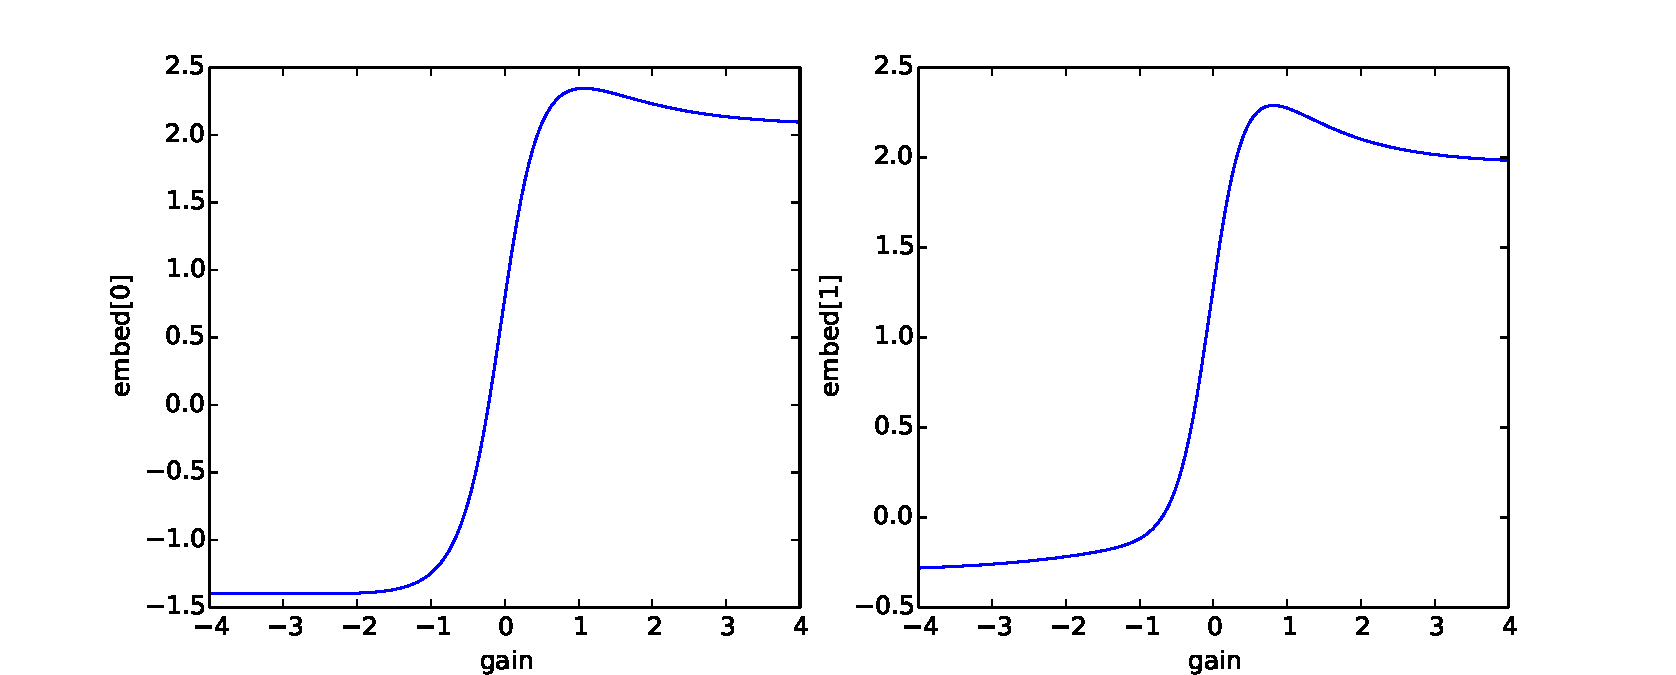
\includegraphics[width=\textwidth]{pointmass_embed_mapping.pdf}
\caption{
Learned mapping from gain factor $g$ to two-dimensional embedding space in point-mass environment.
}
\label{fig:embed-mapping}
\end{figure}
Figure~\ref{fig:embed-mapping} shows the learned mapping from the gain factor $g$
to the embedding space $\cL$.
\TODO{interpret.}

\begin{figure}
\centering
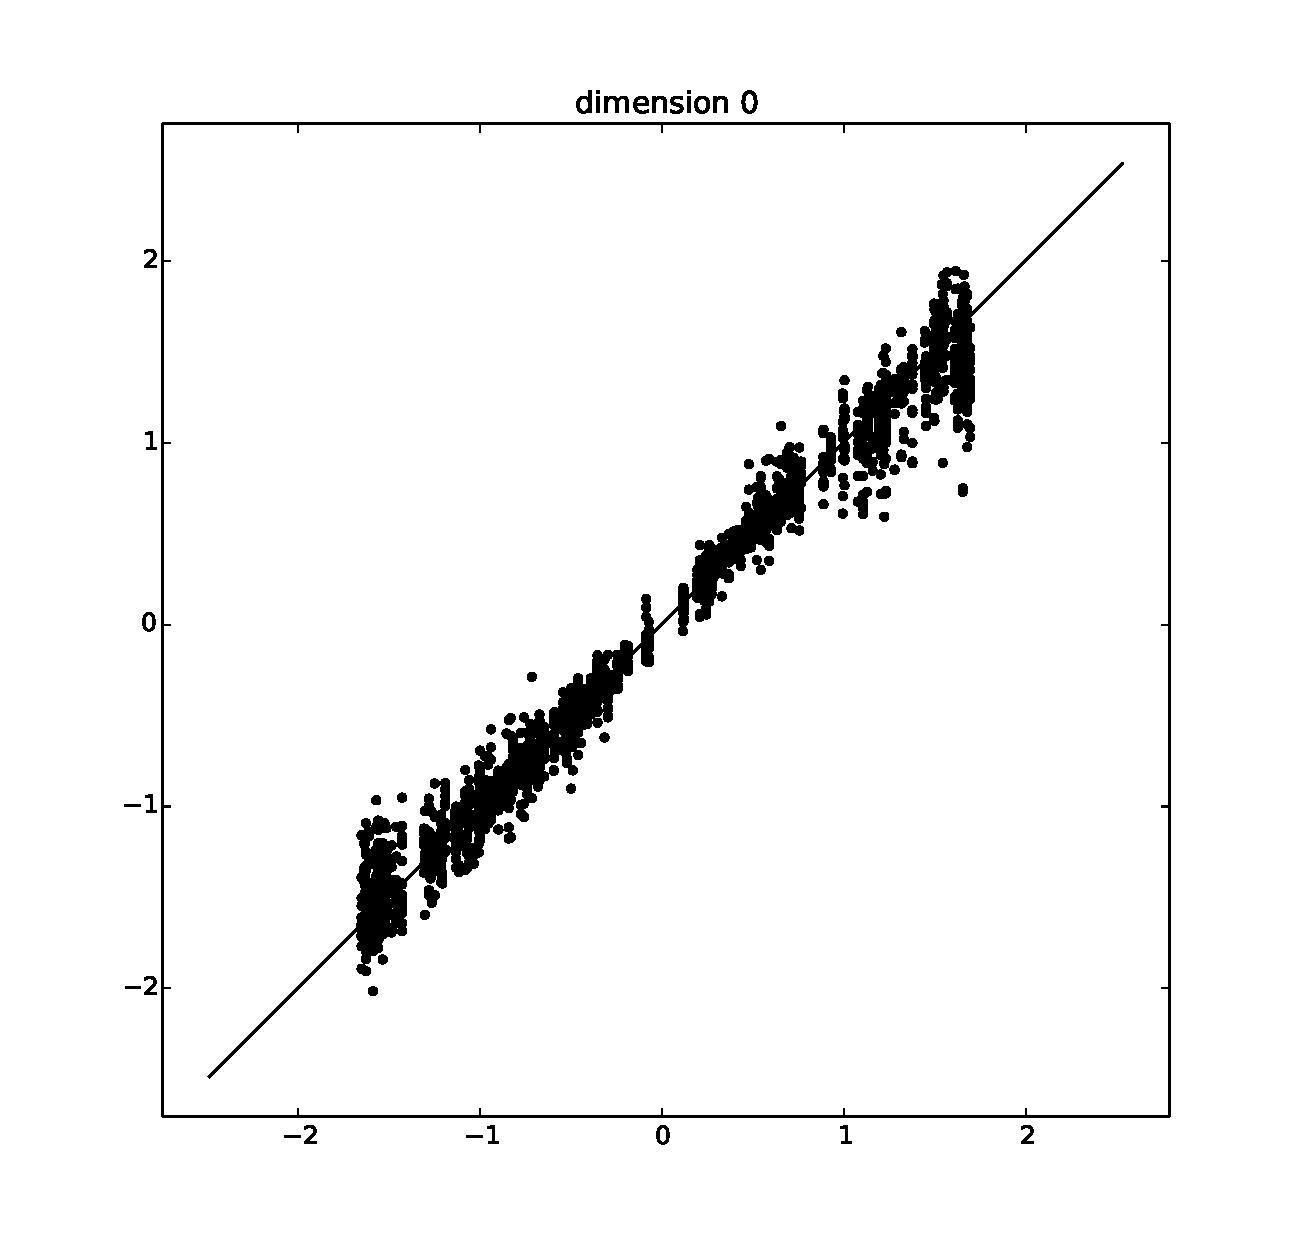
\includegraphics[width=0.45\textwidth]{pointmass_plain_gain_scatter.pdf}
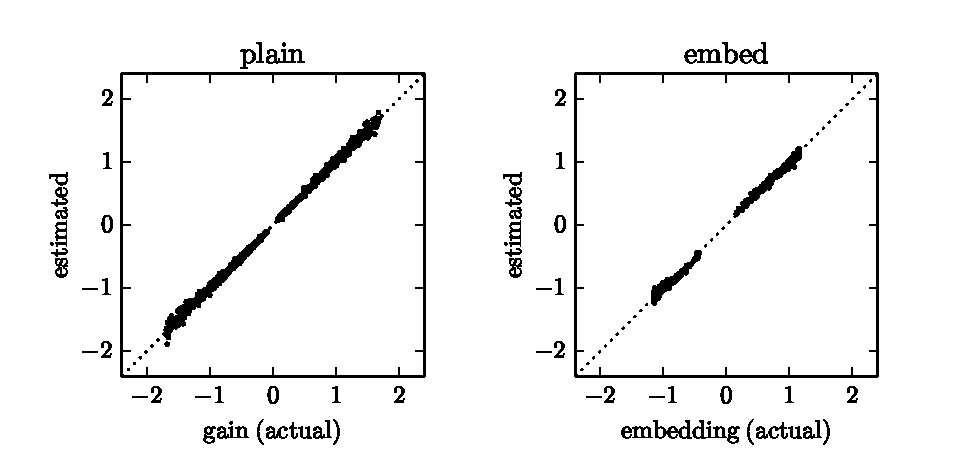
\includegraphics[width=0.45\textwidth]{pointmass_embed_scatter.pdf}
\caption{Scatter plots of actual vs. estimated SysID values.
\emph{Left:} gain parameter $g$ with ``plain'' policy.
\emph{Right:} one of two learned embedding dimensions with ``embed'' policy.
The embedding network separates the gain values into positive and negative clusters.
}
\label{fig:scatter}
\end{figure}
The scatter plots in figure~\ref{fig:scatter} compare the ground truth embedding values gainst those estimated by the inference network in \emph{our} policy, and for the gain factor $g$ against the values estimated by the SysID network in the \emph{plain} policy.
%Against the $x-$axis, density estimates are shown.
These plots illustrate that the learned embedding function ``squashes'' the gain factor $g$ into positive and negative clusters.
The separation between these clusters is magnified, making it easier for the policy to switch between two disjoint behavior styles depending on the sign of the gain factor.
\TODO{can we say anything less wishy-washy? how can we back up this claim?}

\begin{figure}
\centering
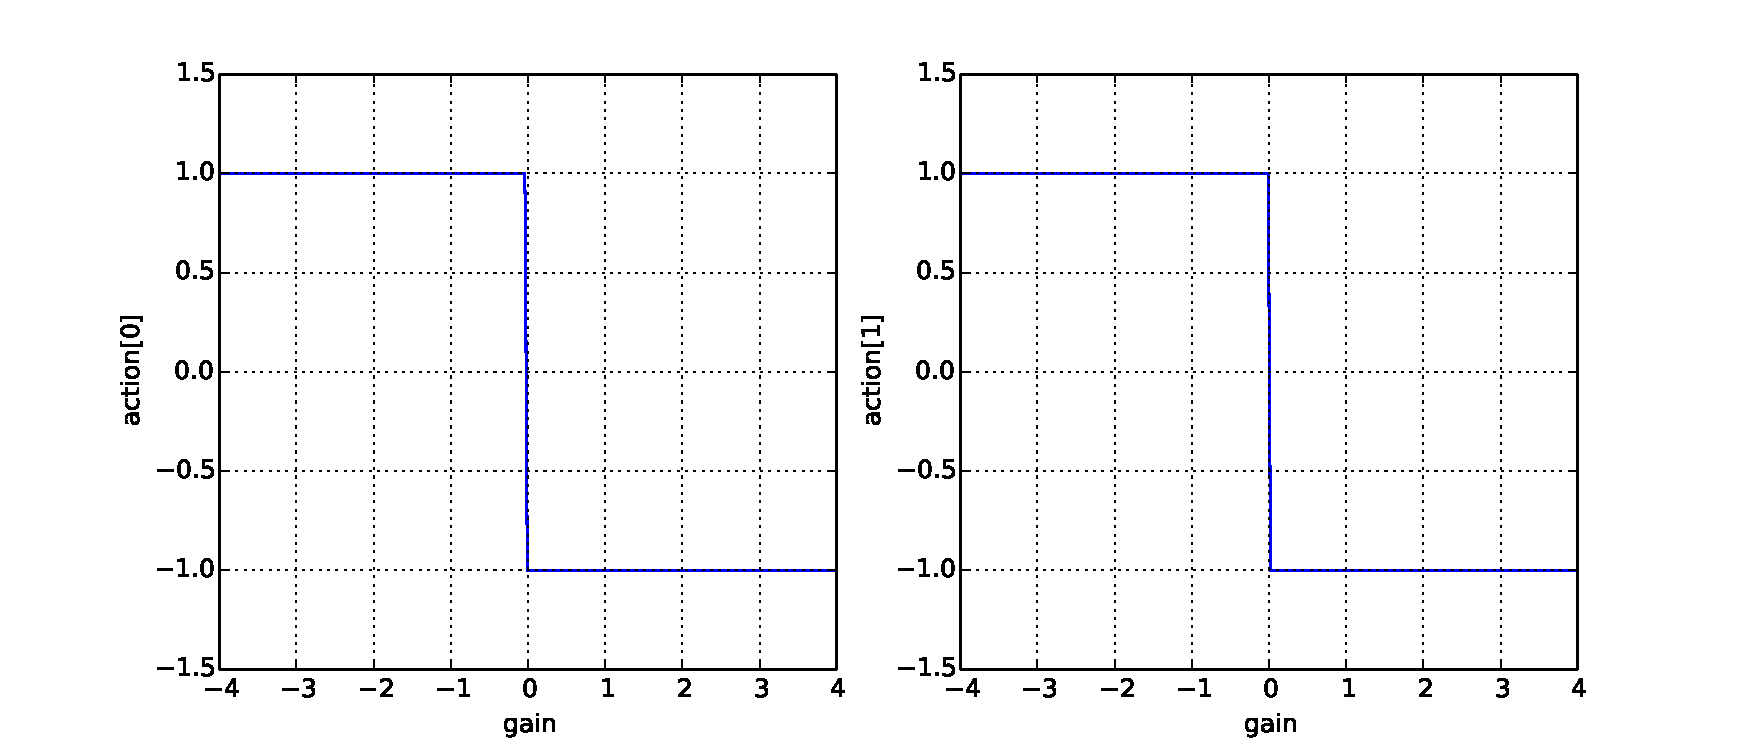
\includegraphics[width=\textwidth]{pointmass_conditional_action.pdf}
\caption{
Action of trained ``embed'' policy at initial state (position $ = (1,1)$, velocity $=(0,0)$) conditioned on gain factor $g$.
Outputs are clipped to valid action range.
Plots show that policy has learned the optimal bang-bang control policy in both positive and negative gain scenarios.
}
\label{fig:conditional_action}
\end{figure}

Figure~\ref{fig:conditional_action} shows the policy output $\pi(a|s_D)$ conditioned on
the gain factor $g$ at the initial task state $s_{t0} = (1, 1)$.

\subsection{More Complex Environment}
\TODO{try a more complex environment}


\subsubsection*{Acknowledgments}

Use unnumbered third level headings for the acknowledgments. All
acknowledgments go at the end of the paper. Do not include
acknowledgments in the anonymized submission, only in the final paper.

\small

\bibliography{bibliography}{}
\bibliographystyle{plainnat}

\end{document}
